\documentclass[../draft.tex]{subfiles}

\begin{document}
    \chapter{Theory}
    \section{Flow Functions}
    In this section, we describe the behavior of the flow functions based on the Jimple language and define semi-formal rules.

    \subsection{Normal Flow}\label{s:normalflow}
    Normal flow functions handle every statement that does not contain an \code{InvokeExpr}. The only case where a new taint can be produced is at an \code{AssignStmt}. It is straight-forward that this is true for statements like \code{IfStmt} if we recall \autoref{s:jimple}. The conditition is either an \code{UnopExpr} or \code{BinopExpr} of which both have no effect on the taint set. But we also skip over \code{IdentityStmt} even though they define a value. This is because we wait for the return site to map all parameters back into the callee.

    Now, lets consider the current statement is an \code{AssignStmt}. It consists of a variable, either a reference or a local, on the left side and an expression on the right side. Jimple ensures we just see one field reference at a time but to reduce the semi-formal rules, we take a shortcut here. So our assigment has the structure $x.f^n \leftarrow y.g^m$ with $n,m \in \{0,1\}$ modelling a possible field reference. Note that the taints can have an access path of an arbitrary length $k$ which is denoted as $h^k$.

    First, we look at the case when the access path matches exactly. Either we have a local ($n=0$) or a field reference ($n=1$) on the left. In the first case, the base of our taint needs to match and in the latter, the first field must also match. If the field references another heap object, we might encounter a non-empty access path $h^k$. This access path needs to be added to the newly created taint. We conclude:
    \begin{itemize}
        \item[] \textbf{Rule 1:} An incoming taint $t = x.f^n.h^k$ with $k \geq 0$ produces the outflowing taint set $T = \{y.g^m.h^k\}$.
    \end{itemize} 

    Next, we might encounter a whole object tainted. In this case, just the base needs to match but the left side is also kept alive because other fields also might be tainted if the object has more than one field.
    \begin{itemize}
        \item[] \textbf{Rule 2:} An incoming taint $t = x.*$ with $k \geq 0$ produces the outflowing taint set $T = \{y.g^m.*, t\}$.
    \end{itemize} 

    Lastly, the right side could also be tainted. This rule is equivalent to the default behaivor but is important later when we consider aliasing in \autoref{s:aliasing}.
    \begin{itemize}
        \item[] \textbf{Rule 3:} An incoming taint $t = y.g^m.h^k$ with $k \geq 0$ produces the outflowing taint set $T = \{t\}$.
    \end{itemize}


    Whenever the taint neither matches on the left nor on the right side, we propagate it further untouched.

    Rule 1 and Rule 3 also work with $*$ appended.

    \subsection{Call Flow}
    For call statements, we have statements of the structure $o.m(a_0, ..., a_n)$ with $n \in \mathbb{N}$. $a_i$ denotes the $i$-th argument, $p_i$ the $i$-th parameter and $c$ the class the method is defined in.

    If we encounter a tainted argument in the caller, the taint need to go through the callee. Due to the backwards direction this is only true for heap objects because only they have references. For primitives or strings we already know the tainted value is not visible in the callee.
    \begin{itemize}
        \item[] \textbf{Rule 1:} An incoming taint $t = a_i.h^k$ with $k \geq 0 \land 0 \leq i \leq n \land \text{typeof}(a_i) \in \mathit{HeapTypes}$ produces the outflowing taint set $T = \{p_i.h^k\}$.
    \end{itemize}

    If the object the method is called on is tainted, the tainted path is visible inside the callee. The callee must be not static.
    \begin{itemize}
        \item[] \textbf{Rule 2:} An incoming taint $t = o.h^k$ with $k \geq 0$ produces the outflowing taint set $T = \{\mathit{this}_c.h^k\}$. 
    \end{itemize}
    
    Tainted static fields are propagated untouched and unconditionally in the callee as they are always visible.
    \begin{itemize}
        \item[] \textbf{Rule 3:} An incoming taint $t = S.h^k$ with $k \geq 0$ produces the outflowing taint set $T = \{t\}$. 
    \end{itemize}

    Next, if the call statement is also an assign statement and the left side is tainted we also need to taint the return value. Methods can have multiple return statements and as we traverse the reversed interprocedural control flow graph, we need to taint all possible return values. The structure of the statement is in this case $x \leftarrow o.m(a_0,...,a_n)$. $r_i$ denotes a return value. $n$ is the number of return statements in the callee. 
    \begin{itemize}
        \item[] \textbf{Rule 4:} An incoming taint $t = x.h^k$ with $k \geq 0$ produces the outflowing taint set $T = \left\{r_i.h^k \mid 0 \leq i < n \right\}$. 
    \end{itemize}

    The taint is killed if it is not matched inside a rule. Instead, it is propagated over the call statement in the CallToReturn flow function.
    \subsection{Return Flow}
    All taints reaching the end of a callee need to be mapped back into the caller. The statement is of the structure $o.m(a_0, ..., a_n)$ with $n \in \mathbb{N}$. $a_i$ denotes the $i$-th argument, $p_i$ the $i$-th parameter and $c$ the class the method is defined in.

    First, we match rule 1 of call flow and map all parameters back into the caller. This time even primitives are mapped back because if we find a tainted value at the start of the method it had to be passed as an argument into the method.
    \begin{itemize}
        \item[] \textbf{Rule 1:} An incoming taint $t = p_i.h^k$ with $k \geq 0 \land 0 \leq i \leq n$ produces the outflowing taint set $T = \{a_i.h^k\}$.
    \end{itemize}

    The $\mathit{this}$ reference is visible in the caller. This is the reverse of rule 2 in call flow.
    \begin{itemize}
        \item[] \textbf{Rule 2:} An incoming taint $t = \mathit{this}_c.h^k$ with $k \geq 0$ produces the outflowing taint set $T = \{o.h^k\}$. 
    \end{itemize}
    
    Tainted static fields are also mapped back untouched and unconditionally equivalent to rule 3 in call flow.
    \begin{itemize}
        \item[] \textbf{Rule 3:} An incoming taint $t = S.h^k$ with $k \geq 0$ produces the outflowing taint set $T = \{t\}$. 
    \end{itemize}

    The taint is killed if it is not matched in a rule.
    \subsection{CallToReturn Flow}
    As already seen in call flow, not every taint is visible inside a callee. 
    Again, the statement structure is $o.m(a_0, ..., a_n)$ with $n \in \mathbb{N}$. $a_i$ denotes the $i$-th argument.

    If the taint neither matches an argument nor the object the method is called on, it is not visible in the callee. Static fields are always visible and thus can not propagated over a statement.
    \begin{itemize}
        \item[] \textbf{Rule 1:} An incoming taint $t = x.h^k$ with $k \geq 0 \land (\forall a \in \mathit{Arguments}: a \neq x) \land x \neq o \land x \notin \mathit{Static}$ produces the outflowing taint set $T = \{t\}$. 
    \end{itemize}

    If a taint is limited to its base, so no fields are tainted, the taint is also propagated over the statement as the reference is passed by copy-by-value and assigments to the parameter overwrites the reference in the callee but has no effect on the reference in the caller.
    \begin{itemize}
        \item[] \textbf{Rule 2:} An incoming taint $t = a_i$ with $0 \leq i \leq n$ produces the outflowing taint set $T = \{t\}$. 
    \end{itemize}
        

    \section{Complexity of Data Flow Analysis}
    IFDS has a time-complexity of $O(E \cdot D^3)$. The edges in the control-flow graph are set by the to-be-analyzed app. The domain depends on the tainted variables observed by the IFDS search. Arzt et al evaluation of \textsc{FlowDroid} shows no correlation between a-priori known parameters and the runtime \cite{Arzt2017PhD}. So, we are left with the number of taint propagations as the only parameter correlated to the runtime but they are only known afterwards. 

    The number of taint propagations depends on two factors: the lifetime of taints and the number of taints. Both factors highly depend on the search direction which we will explain in the following paragraphs.

    Starting with the number of taints, we

    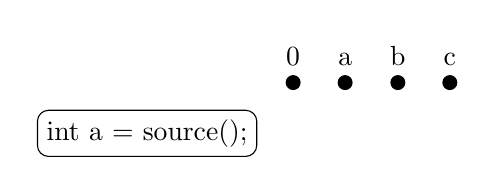
\begin{tikzpicture}[auto, 
        s/.style={draw, rounded corners},
        v/.style={draw, fill=black, circle, inner sep=0pt, minimum size=5pt},
        every node/.style={align=center},
        every matrix/.style={ampersand replacement=\&,column sep=0.25cm,row sep=.25cm}]
        \matrix {
            \& \node[v, label={0}] (zero1) {}; \& \node[v, label={a}] (a1) {}; \& \node[v, label={b}] (b1) {}; \& \node[v, label={c}] (c1) {};\\
            \node[s] (s1) {int a = source();}; \& \& \& \&\\
            % \& \node[v] (zero2) {}; \& \node[v] (a2) {}; \& \node[v] (b2) {}; \& \node[v] (c2) {};\\
            % \node[s] (s2) {int b = a;}; \& \& \& \&\\
            % \& \node[v] (zero3) {}; \& \node[v] (a3) {}; \& \node[v] (b3) {}; \& \node[v] (c3) {};\\
            % \node[s] (s3) {int c = b;}; \& \& \& \&\\
            % \& \node[v] (zero4) {}; \& \node[v] (a4) {}; \& \node[v] (b4) {}; \& \node[v] (c4) {};\\
            % \node[s] (s4) {leak(c);} \& \& \& \&\\
            % \& \node[v] (zero5) {}; \& \node[v] (a5) {}; \& \node[v] (b5) {}; \& \node[v] (c5) {};\\
        };

        % \draw[sto] (s1) -- (s2);
        % \draw[sto] (s2) -- (s3);
        % \draw[sto] (s3) -- (s4);

        % \draw[vto] (zero1) -- (zero2);
        % \draw[vto] (zero2) -- (zero3);
        % \draw[vto] (zero3) -- (zero4);
    \end{tikzpicture}

    

    Explain where the run-time comes from.
    Depends the number of edge propagations
    \begin{itemize}
        \item "Branching factor" might be different for forwards/backwards, with some simple examples?
            \begin{itemize}
                \item  tainted = a + b. BW we don't know which was responsible for the tainted c $\rightarrow$ 2 new taints
                \item Simple assigments in a strict r-to-l order: a = b. FW {a, b} while BW we can kill a and just go with {b}
            \end{itemize}
        \item Lifetime of taints 
        \begin{itemize}
            \item Static taints are valid everywhere
            \item Best practise "sanitize just before displaying" might favor backwards
        \end{itemize}
        \item Number of taints
        \begin{itemize}
            \item There seems to be no correlation between source count and analysis time
            \item Probably also holds for sinks?
            \item There might be indicator for a single app whether it is better to start at sources or sinks
        \end{itemize}


    \end{itemize}

\end{document}